\section{Equipment}

\subsection{CubeSat Components}
\subsubsection{PCB-printed-magnetorquer-integrated solar panels developed by LED Dynamics}
\begin{description}
\item[Cost] 3,000.00 USD
\item[Description] Provide charging power to the EPS
\item[Description] Provide de-tumbling and pointing actuation through
  integrated magnetorquers
\end{description}

\subsubsection{Inertial Measurement Unit (IMU)}
\begin{description}
\item[Cost] 0.00 USD
\item[Description] MEMS gyroscope with accelerometer, magnetometer and
  Adaptive Kalman Filter to determine inertial reference frame
\end{description}

\subsubsection{GPS Board}
\begin{description}
\item[Cost] 7,980.00 USD
\item[Description] L1 GPS for absolute positioning
\end{description}

\subsubsection{GPS Patch Antenna}
\begin{description}
\item[Cost] 200.00 USD
\item[Description] Antcom L1 GPS antenna P/N 1.5G15A
\end{description}

\subsubsection{Radio Receiver}
\begin{description}
\item[Cost] 5,000.00 USD
\item[Description] Astrodev Lithium
\item[Description] For ground station and sat-to-sat communication
\end{description}

\subsubsection{Radio Antenna}
\begin{description}
\item[Cost] 6,500.00 USD
\item[Description] ISIS CubeSat Antenna System
\item[Description] For radio transmission
\end{description}

\subsubsection{Electric Power System}
\begin{description}
\item[Cost] 5,000.00 USD
\item[Description] CubeSatKit Battery Module 2 special manufacture
\end{description}

\subsubsection{Skeletonized Walls}
\begin{description}
\item[Cost] 925.00 USD
\item[Description] CubeSatKit Chassis Walls, PC104 supported
\end{description}

\subsubsection{AntS Top Plate}
\begin{description}
\item[Cost] 725.00 USD
\item[Description] Top plate with AntS integration, PC104
\end{description}

\subsubsection{Baseplate}
\begin{description}
\item[Cost] 525.00 USD
\item[Description] CubeSatKit manufactured
\item[Description] Benchmark thruster compatible
\item[Description] Ejection tabs
\end{description}

\subsubsection{CPU Board}
\begin{description}
\item[Cost] 5,500.00 USD
\item[Description] BeagleBoneBlack
\end{description}

\subsubsection{Camera System}
\begin{description}
\item[Cost] 0.00 USD
\item[Description] Photograph CubeSats in formation
\end{description}


\subsection{Test Equipment}

\subsubsection{Thermal Vacuum Chamber}
\begin{description}
\item[Cost] 0.00 USD
\item[Description] To test CubeSat integrity in environmental
  conditions encountered in space
\end{description}

\subsubsection{Shaker Table}
\begin{description}
\item[Cost] 0.00 USD
\item[Description] To test CubeSat integrity during rocket launch
\end{description}

\begin{figure}
\centering
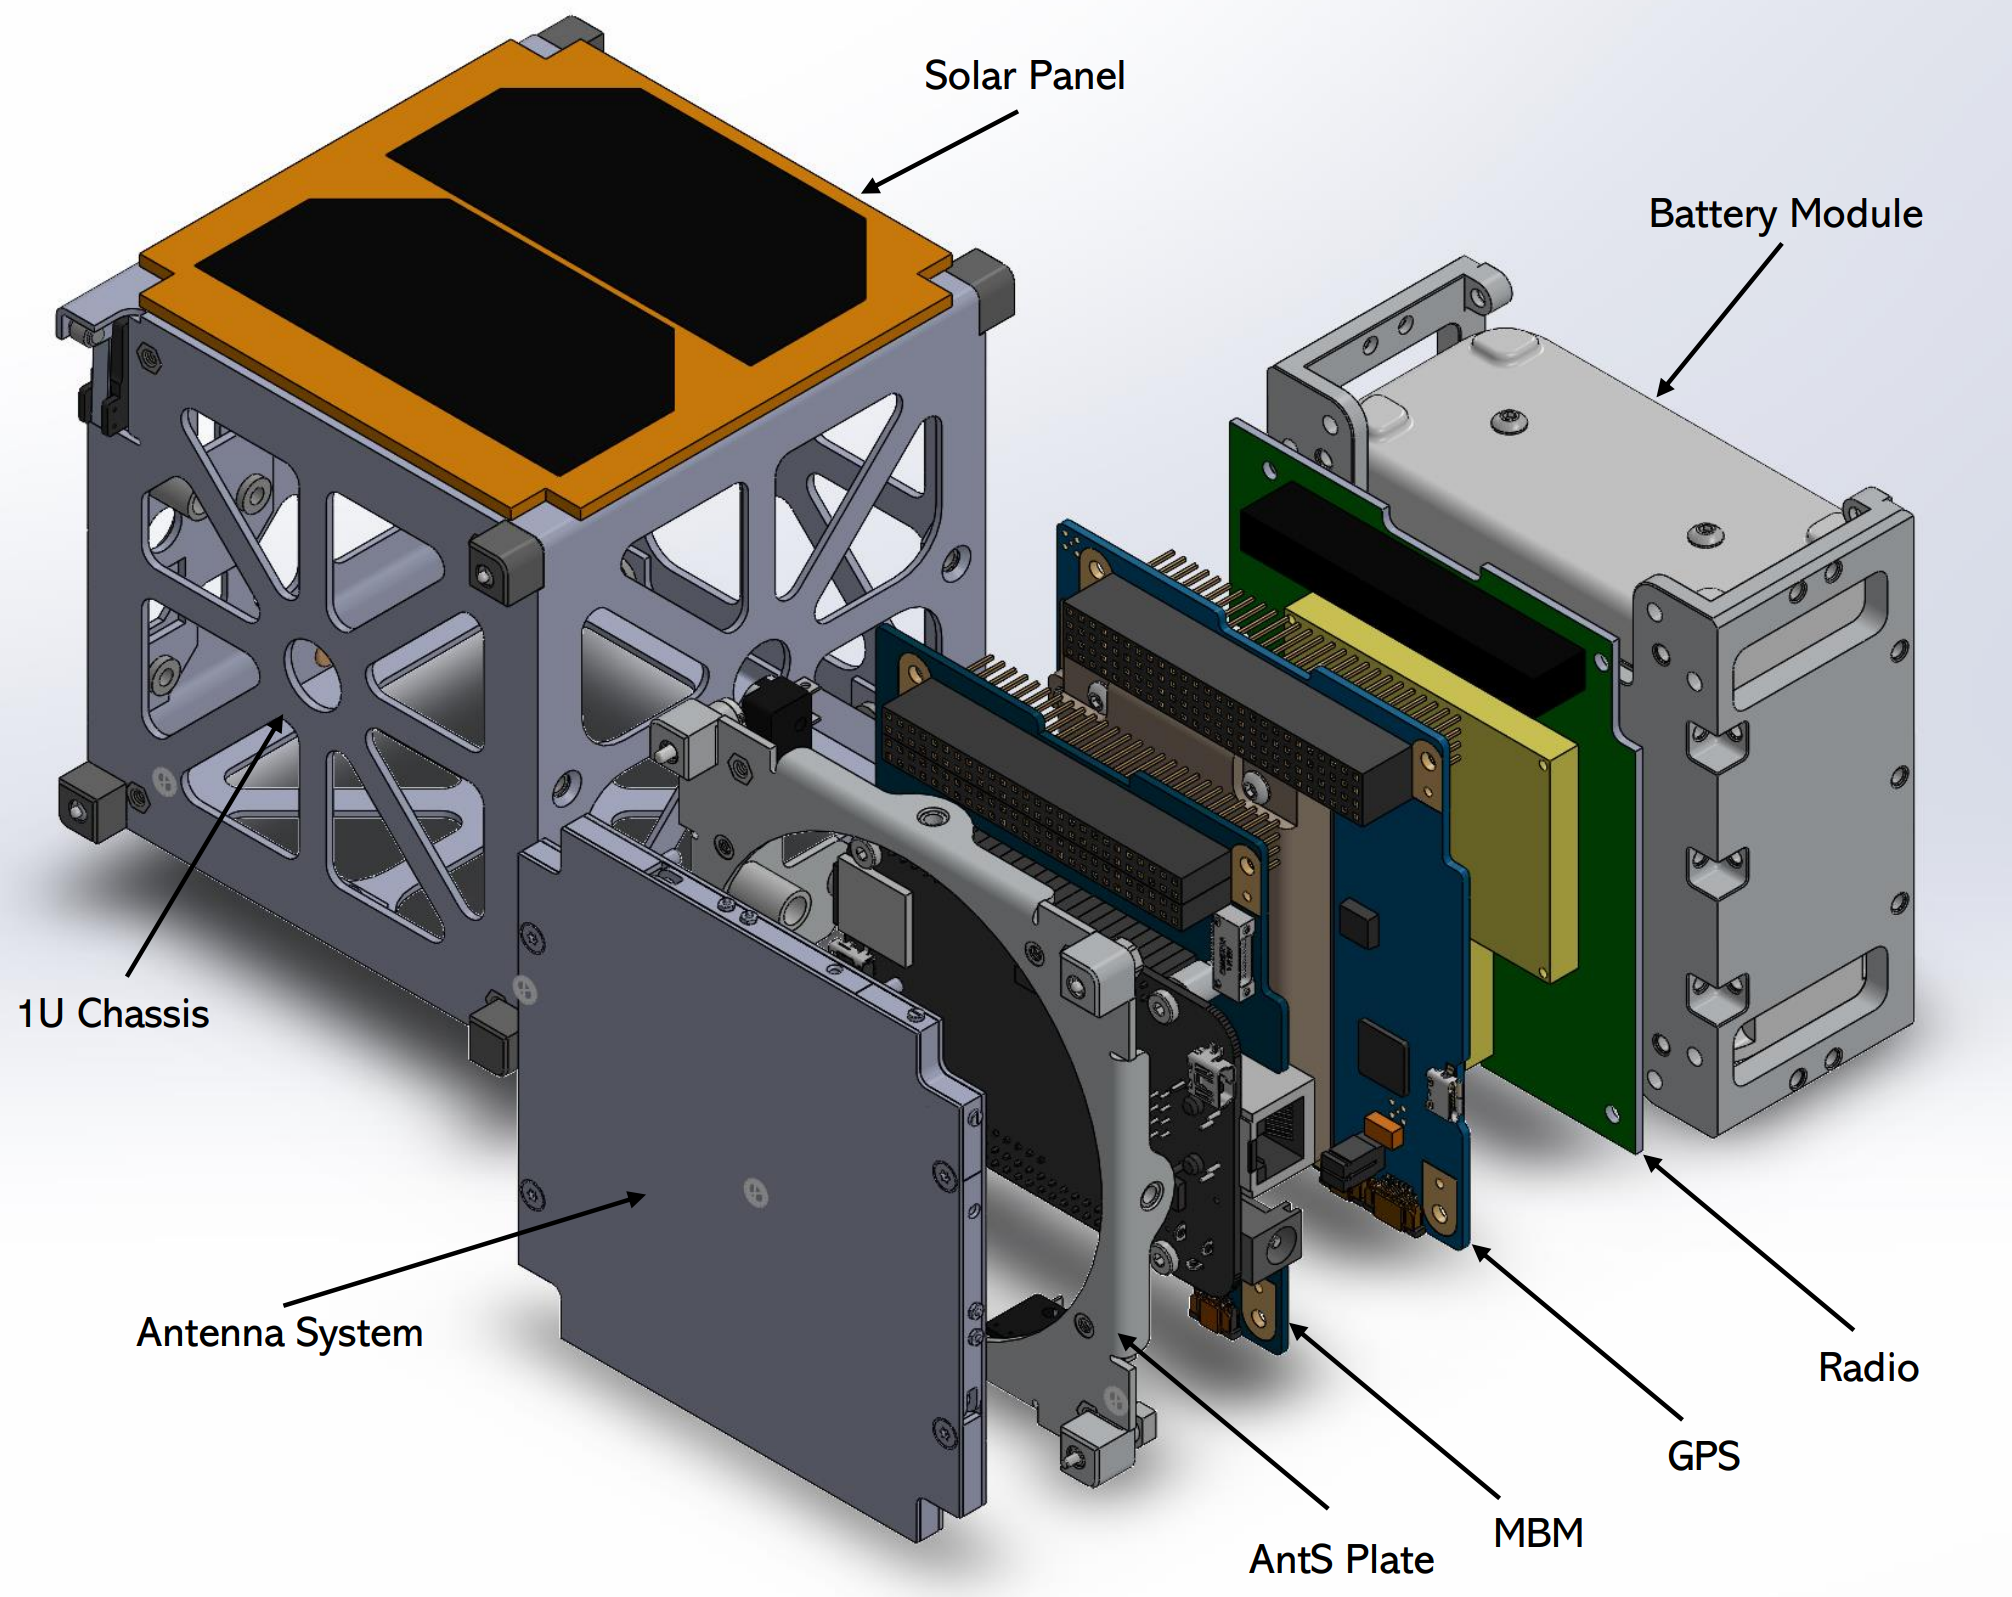
\includegraphics[width=\textwidth]{cubesat-model}
\caption{Expanded view of proposed CubeSat model. \textit{Note:
    Benchmark thruster not included to avoid divulging IP.}}
\label{fig:cubesat-model}
\end{figure}
